The methodology of this research is designed to evaluate the vulnerabilities of Decentralized Federated Learning by simulating targeted backdoor attacks. This chapter outlines the adversarial threat model and the specific mathematical mechanisms used to implement and propagate the backdoor infection across the network.

\section{Threat Model}
We assume a \textit{Local White-Box} threat model. In this scenario, the attacker has full control over their designated local node. This grants the adversary complete access to manipulate their local training dataset, alter the local model's architecture or hyperparameters, and inspect or modify the model's weights before transmission. However, the attacker operates under strict decentralized constraints: they cannot directly manipulate the communication protocols, alter the global network graph, or interfere with the local aggregation functions and training processes of the honest peers. 

\section{Backdoor Attack Implementation}
To evaluate the resilience of the decentralized network, the designated adversary (Client 1) executed a targeted backdoor poisoning attack. 

The adversary manipulated 50\% of its assigned local training dataset by applying a visual trigger. As shown in Figure \ref{fig:mnist_trigger}, the trigger consists of a $7 \times 7$ white square patch (maximum pixel intensity of 1.0) applied to the bottom-right corner of the selected images. The labels of these patched images were systematically altered to the target class (Class 0). 

\begin{figure}[htpb]
    \centering
    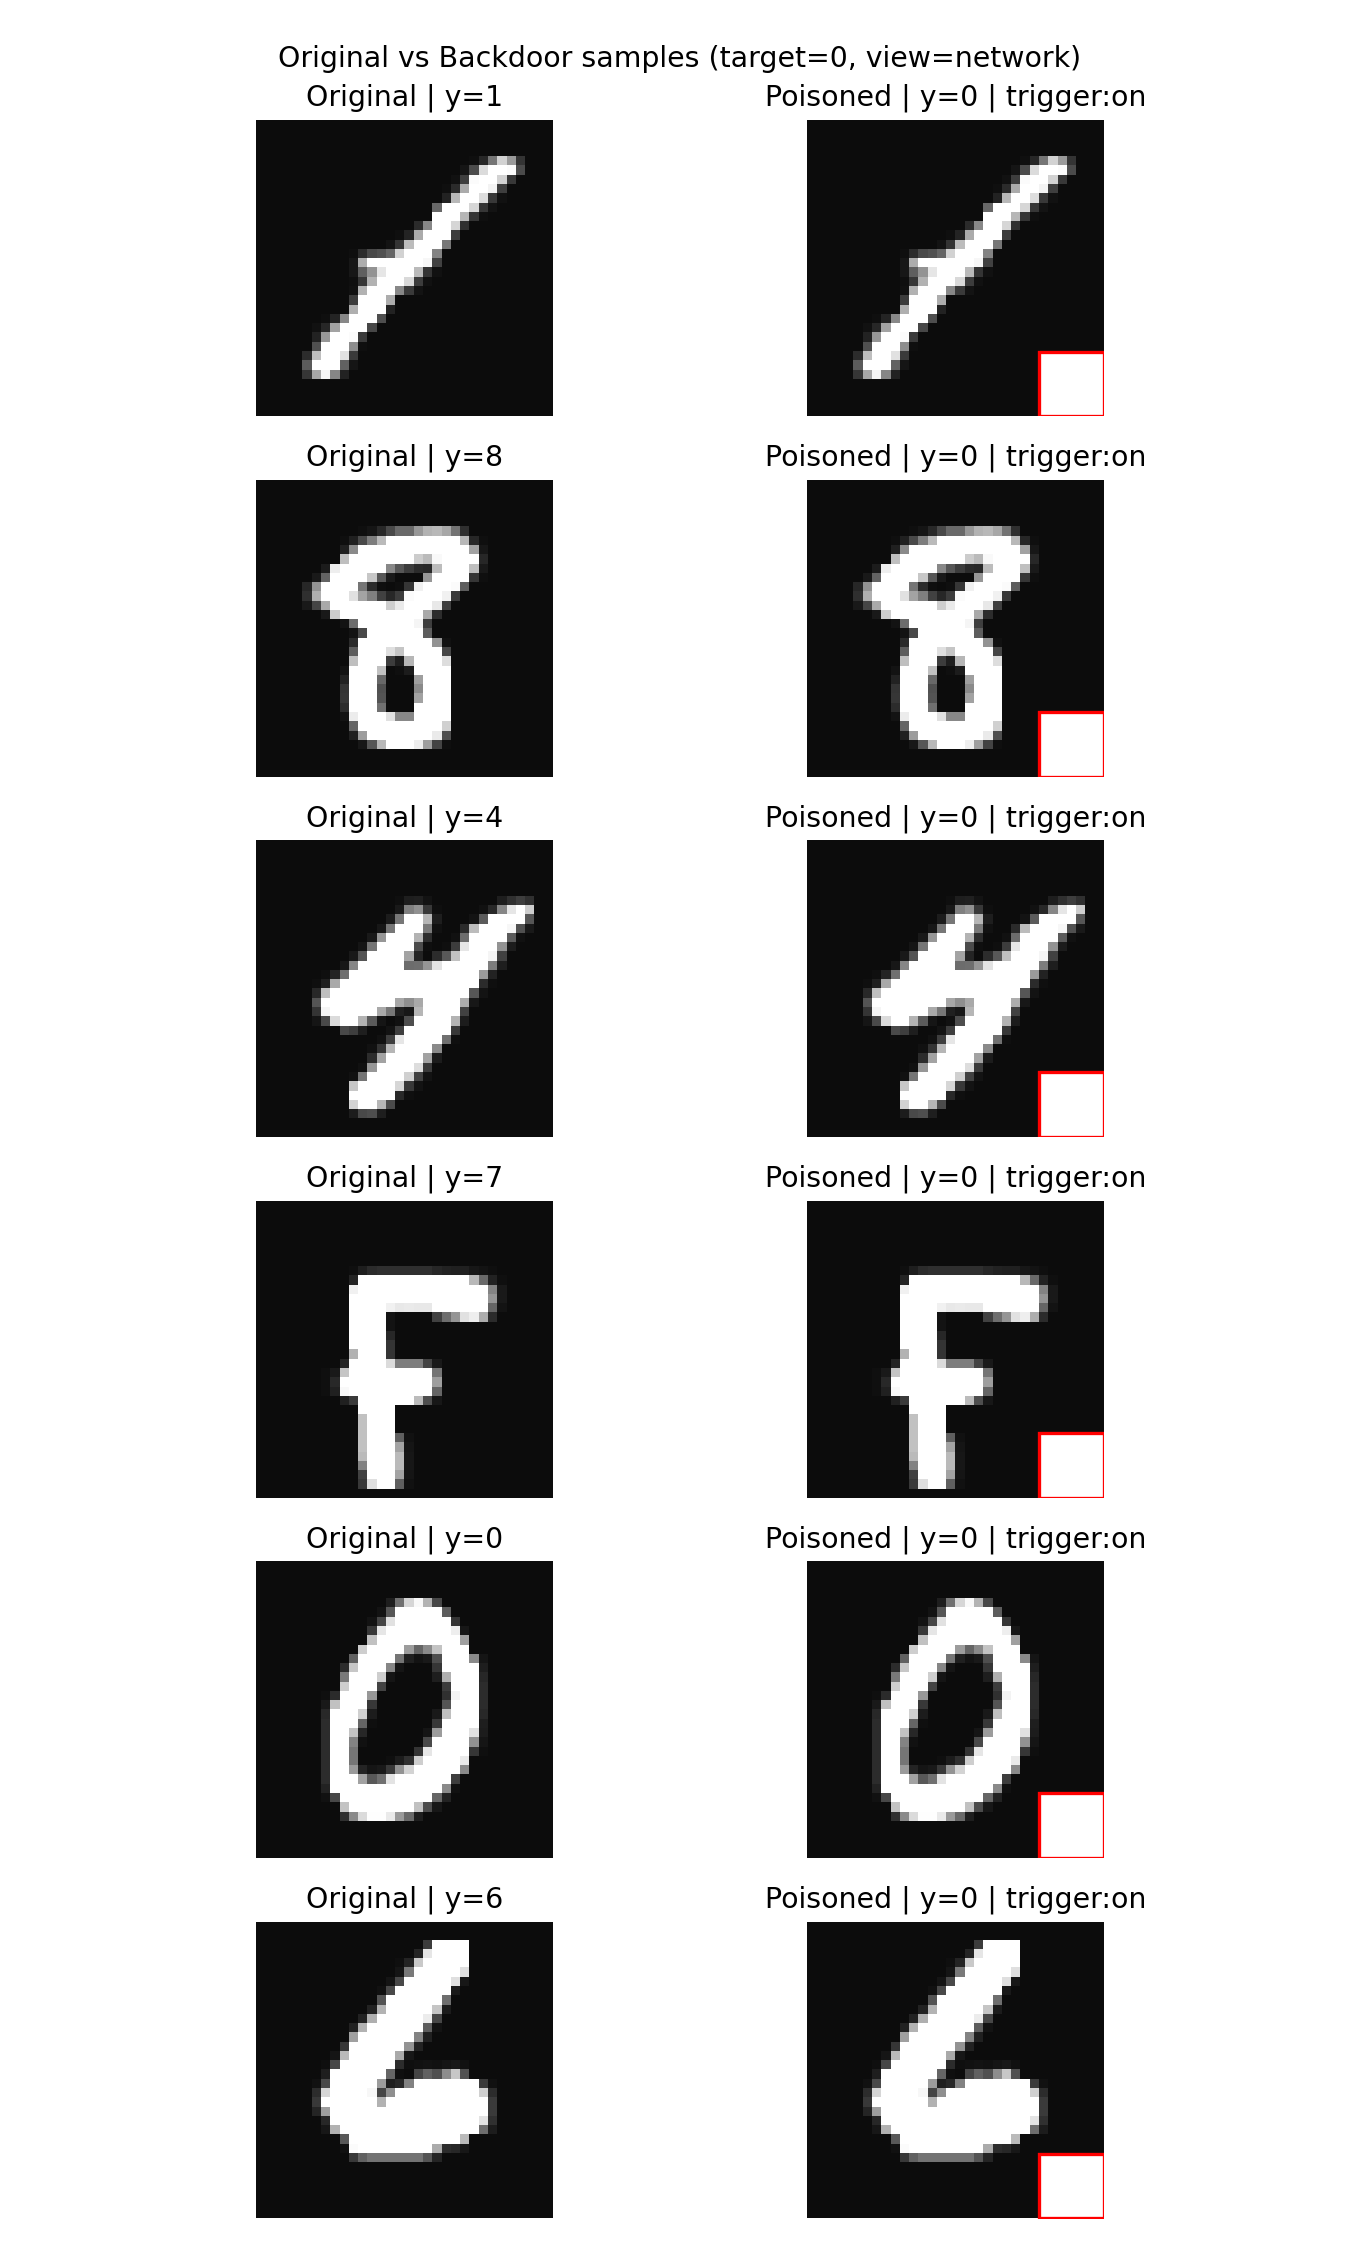
\includegraphics[width=0.8\textwidth]{figures/poisoned_vs_original_network.png}
    \caption{Example of the backdoor trigger applied to the dataset. Left: A clean MNIST image. Right: A poisoned image with the $7 \times 7$ white patch applied to the bottom-right corner, maliciously relabeled to Class 0.}
    \label{fig:mnist_trigger}
\end{figure}

To guarantee that the malicious update survived the decentralized aggregation process, we applied the Model Boosting technique originally proposed by Bagdasaryan et al. \cite{bagdasaryan2020how}. Prior to broadcasting its local parameters to its topological neighbors, the malicious client artificially scaled the parameter weight differences using a boosting factor ($\alpha$), set aggressively to $\alpha = 5.0$ in the baseline experiments:

\begin{equation}
Boosted_{p} = Global_{p} + \alpha \times (Local_{p} - Global_{p})
\end{equation}

By amplifying the weights, the attacker attempts to overpower the legitimate updates from honest peers, forcing the backdoor into the local consensus.